\graphicspath{{appendices/figures}}

\chapter{Anexo: Manual de Usuario}\label{appendix:manual}

En este anexo se presenta el manual de usuario del programa disponible en el siguiente repositorio de GitHub: \href{https://github.com/franciscoaguirre/voxel-cone-tracing}{https://github.com/franciscoaguirre/voxel-cone-tracing}.

El repositorio incluye un ejecutable localizado en la carpeta \textit{bin}, bajo el nombre \textit{cli}. Cabe destacar que dicho ejecutable es compatible únicamente con sistemas operativos Linux. En caso de emplear un sistema operativo diferente, será necesario compilar el ejecutable a partir del código fuente proporcionado.

\subsection{Compilación del Código Fuente}

Para compilar el código fuente, es indispensable tener instalado \href{Rust}{https://rustup.rs/}. Una vez instalado, la compilación se realiza mediante la ejecución del siguiente comando:

\texttt{cargo build --release}

\section{Opciones de Ejecución}

Si se ejecuta el programa sin especificar ninguna opción, este finalizará inmediatamente. Es necesario indicar qué escena se desea utilizar. En la carpeta \textit{scenes} se encuentran varios archivos de escena con la extensión \textit{.ron}. Para ejecutar una escena específica, debe añadirse la opción \texttt{--scene <nombre-escena>} al comando de ejecución, donde ``<nombre-escena>'' corresponde al nombre del archivo de la escena, sin incluir la extensión. Por ejemplo:

\texttt{./cli --scene cornell-box}

Además, el programa utiliza configuraciones definidas en el archivo \textit{config.ron}, donde se pueden ajustar parámetros como la resolución de la ventana y la resolución de la grilla de vóxeles.

El repositorio también incluye archivos de \textit{presets}, los cuales proporcionan un estado inicial para las escenas. Aunque se proporcionan algunos ejemplos generados automáticamente, más adelante se detallará cómo generar nuevos.

\section{Controles del Programa}

Una vez dentro del programa, con una escena cargada y sin un \textit{preset} activado, se pueden utilizar las teclas \textit{W}, \textit{A}, \textit{S}, \textit{D} o las flechas del teclado para mover la cámara. A continuación, se describen algunas de las funcionalidades clave:

\begin{itemize}
    \item Tecla \textit{1}: Muestra la escena cargada.
    \item Tecla \textit{2}: Muestra la versión voxelizada de la escena.
    \item Tecla \textit{C}: Permite mover la fuente de luz, representada por un cubo blanco vacío. Los efectos de la luz se visualizarán cuando se activen opciones de iluminación directa o indirecta desde el menú.
\end{itemize}

\subsection{Acceso al Menú}

El menú principal se accede mediante la tecla \textit{Escape}, y proporciona acceso a varios submenús para el control detallado de diferentes aspectos del programa.

\begin{figure}[h]
    \centering
    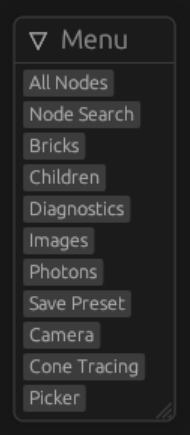
\includegraphics[width=.5\textwidth]{menu.png}
    \caption{Menú Principal.}
    \label{fig:menu}
\end{figure}

Como se observa en la figura \ref{fig:menu}, los submenús disponibles son:

\begin{itemize}
	\item All Nodes
	\item Node Search
	\item Bricks
	\item Children
	\item Diagnostics
	\item Images
	\item Photons
	\item Save Preset
	\item Camera
	\item Cone Tracing
	\item Picker
\end{itemize}

A continuación, se describen en detalle cada uno de estos.

\subsubsection{All Nodes}

Este submenú permite visualizar la representación gráfica del \textit{octree} y ajustar el nivel de detalle mostrado. En la figura \ref{fig:all_nodes} se muestra el botón que activa la visualización del \textit{octree} y el \textit{slider} que permite controlar los niveles.

\begin{figure}[h]
    \centering
    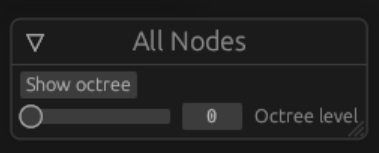
\includegraphics[width=.5\textwidth]{all_nodes.png}
    \caption{Submenú \textit{All Nodes}.}
    \label{fig:all_nodes}
\end{figure}

\subsubsection{Node Search}

Este submenú ofrece la funcionalidad de buscar nodos del \textit{octree} ya sea por índice o posición. Al seleccionar un nodo de la lista, este se muestra en el espacio de la escena. Además, existe la opción de destacar los nodos vecinos al nodo seleccionado, y es posible seleccionar múltiples nodos. Este menú ha sido de gran utilidad durante el proceso de depuración del programa. La figura \ref{fig:node_search} ilustra su uso.

\begin{figure}[h]
    \centering
    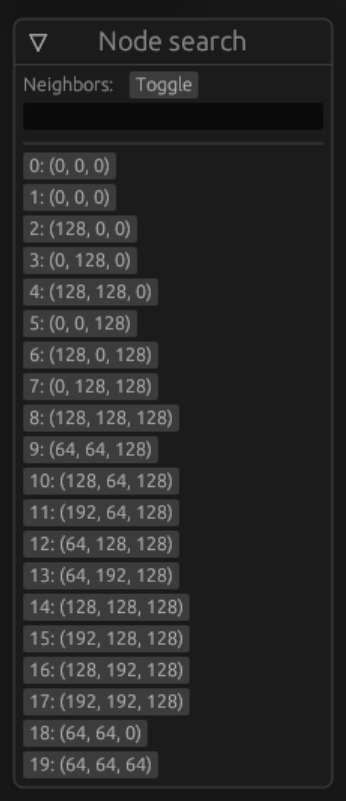
\includegraphics[width=.5\textwidth]{node_search.png}
    \caption{Submenú \textit{Node Search}.}
    \label{fig:node_search}
\end{figure}

\subsubsection{Bricks}

Este submenú, a diferencia de los anteriores que muestran nodos, permite visualizar los bricks asociados a esos nodos. La figura \ref{fig:bricks} muestra las distintas opciones disponibles. Para limitar el impacto en el rendimiento, es posible visualizar una capa de vóxeles de los bricks a la vez. Asimismo, se pueden visualizar el color y la irradiancia de los vóxeles, así como las normales de los mismos.

Los controles situados al final del submenú permiten cambiar la dirección desde la cual se observan los bricks, algo relevante dado que los vóxeles son filtrados anisotrópicamente.

\begin{figure}[h]
    \centering
    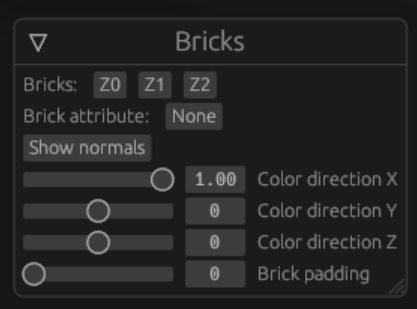
\includegraphics[width=.5\textwidth]{bricks.png}
    \caption{Submenú \textit{Bricks}.}
    \label{fig:bricks}
\end{figure}

\subsubsection{Children}

Al seleccionar un nodo utilizando el submenú \textit{Node Search}, este submenú muestra los atributos del nodo seleccionado. La figura \ref{fig:children} muestra este submenú con y sin un nodo seleccionado. Una vez seleccionado un nodo $n$, se presentan los índices de sus nodos hijos, los cuales pueden ser posteriormente buscados en el submenú \textit{Node Search}.

\begin{figure}[h]
    \begin{center}
    \begin{subfigure}{.49\textwidth}
        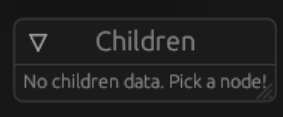
\includegraphics[width=\textwidth]{children-off.png}
        \caption{Sin nodo seleccionado.}
    \end{subfigure}
    \begin{subfigure}{.49\textwidth}
        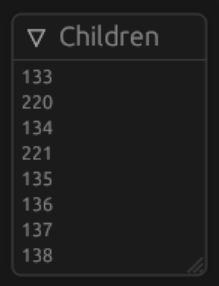
\includegraphics[width=\textwidth]{children-on.png}
        \caption{Con nodo seleccionado.}
    \end{subfigure}
    \caption{Submenú \textit{Children}.}
    \label{fig:children}
    \end{center}
\end{figure}

\subsubsection{Diagnostics}

El submenú \textit{Diagnostics} proporciona información sobre el rendimiento de la aplicación, específicamente los cuadros por segundo (FPS), como se muestra en la figura \ref{fig:diagnostics}.

\begin{figure}[h]
    \centering
    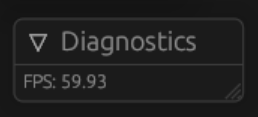
\includegraphics[width=.5\textwidth]{diagnostics.png}
    \caption{Submenú \textit{Diagnostics}.}
    \label{fig:diagnostics}
\end{figure}

\subsubsection{Images}

Este submenú permite mostrar diferentes imágenes en pantalla, de manera similar a cómo las teclas \textit{1} y \textit{2} permiten mostrar la escena original y la versión voxelizada respectivamente. En la figura \ref{fig:images}, se presentan las opciones disponibles:

\begin{itemize}
    \item Color: Muestra la escena original, equivalente a presionar la tecla \textit{1}.
    \item Direct Light: Muestra la escena iluminada únicamente por la luz directa.
    \item Indirect Diffuse: Muestra la escena iluminada por la luz indirecta difusa reflejada en las superficies.
    \item Indirect Specular: Muestra la escena iluminada por la luz indirecta especular reflejada en superficies brillantes o metálicas.
    \item Ambient Occlusion: Muestra la escena en escala de grises de acuerdo con la oclusión ambiental en cada punto.
\end{itemize}

Cada una de estas opciones añade un efecto adicional a la imagen, permitiendo una visualización progresiva de los diferentes elementos de la iluminación.

\begin{figure}[h]
    \centering
    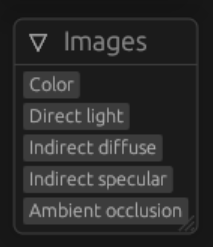
\includegraphics[width=.5\textwidth]{images.png}
    \caption{Submenú \textit{Images}.}
    \label{fig:images}
\end{figure}

\subsubsection{Photons}

Este submenú, similar al submenú \textit{Children}, muestra la cantidad de fotones en cada vóxel del brick de un nodo seleccionado previamente en el submenú \textit{Node Search}.

\subsubsection{Save Preset}

Este submenú permite guardar todas las configuraciones seleccionadas en el menú en un archivo de \textit{preset}.
Para guardar, simplemente se debe elegir un nombre para el archivo y presionar el botón \textit{Save}, como se muestra en la figura \ref{fig:save_preset}.
Estos archivos pueden ser cargados en futuras ejecuciones utilizando la opción \texttt{--preset <nombre-archivo>}.

\begin{figure}[h]
    \centering
    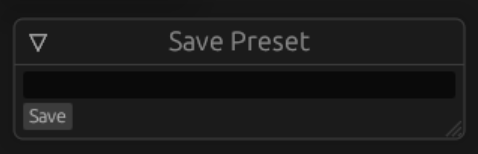
\includegraphics[width=.5\textwidth]{save_preset.png}
    \caption{Submenú \textit{Save Preset}.}
    \label{fig:save_preset}
\end{figure}

\subsubsection{Camera}

Este submenú permite cambiar la proyección de la cámara a una vista ortogonal.

\subsubsection{Cone Tracing}

Este submenú ofrece control sobre la apertura y la distancia máxima de los conos utilizados para sombras, oclusión ambiental, reflexión difusa, reflexión especular y conos de prueba. La figura \ref{fig:cone_tracing} ilustra estas opciones.

\begin{figure}[h]
    \centering
    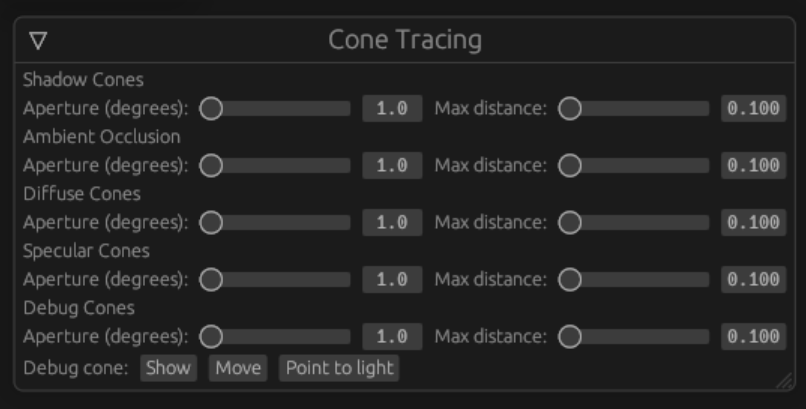
\includegraphics[width=.5\textwidth]{cone_tracing.png}
    \caption{Submenú \textit{Cone Tracing}.}
    \label{fig:cone_tracing}
\end{figure}

\subsubsection{Picker}

Este submenú permite activar un modo en el cual el cursor puede ser utilizado para seleccionar un punto en la pantalla y lanzar un cono desde ese punto en la escena. El submenú se muestra en la figura \ref{fig:picker-menu}, y un ejemplo del cono de prueba en acción se presenta en la figura \ref{fig:picker-action}. El cono de prueba muestra los nodos a través de los cuales pasa.

\begin{figure}[h]
    \centering
    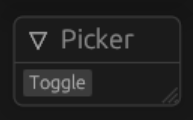
\includegraphics[width=.5\textwidth]{picker-menu.png}
    \caption{Submenú \textit{Picker}.}
    \label{fig:picker-menu}
\end{figure}

\begin{figure}[h]
    \centering
    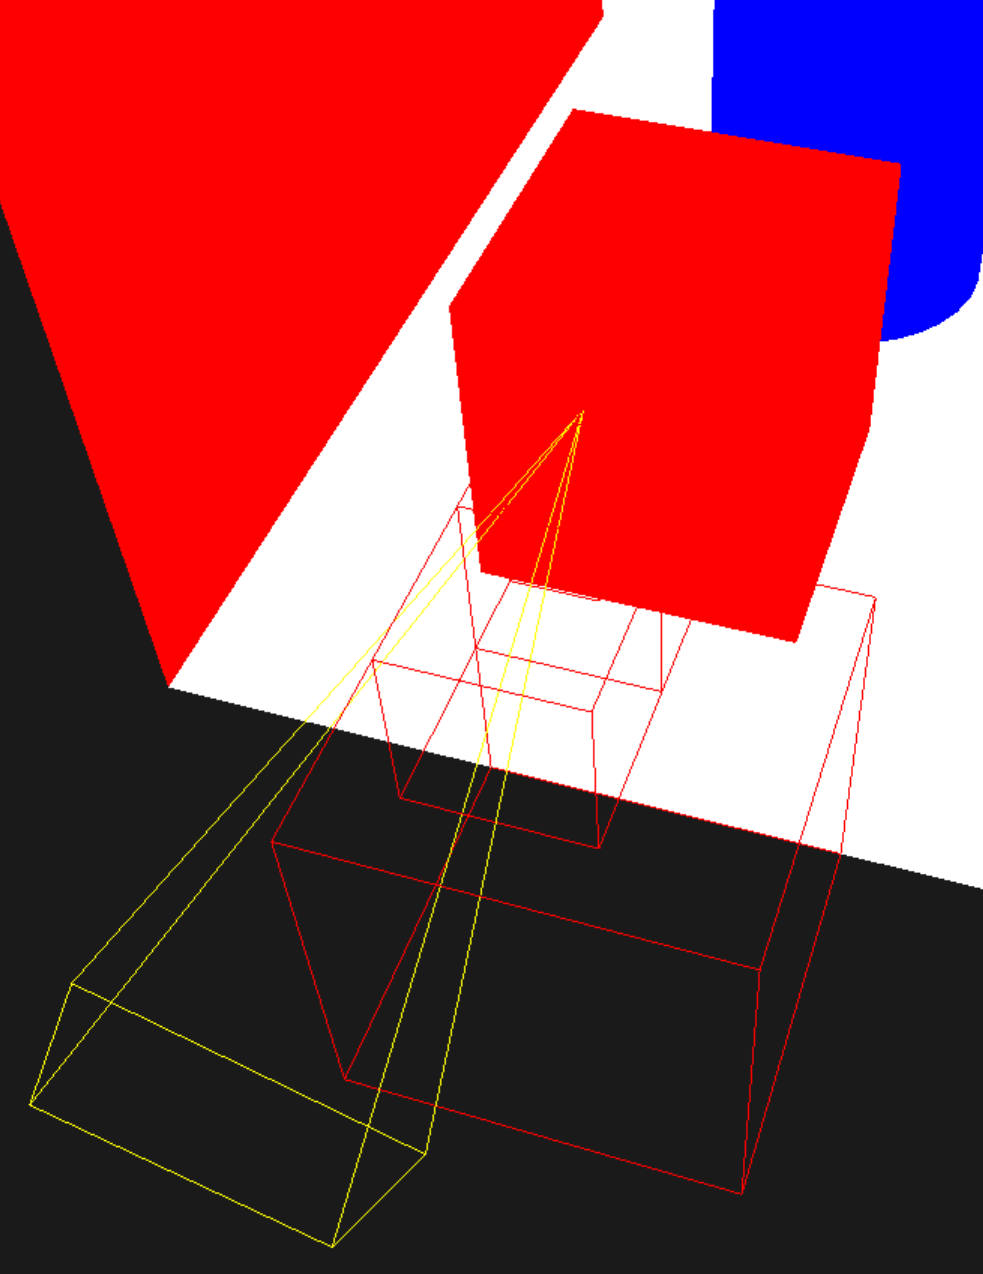
\includegraphics[width=.5\textwidth]{picker-action.png}
    \caption{Cono de prueba en acción.}
    \label{fig:picker-action}
\end{figure}
